\documentclass[12pt,a4paper]{article}

% ── Packages ─────────────────────────────────────────────────────────
\usepackage[utf8]{inputenc}
\usepackage[T1]{fontenc}
\usepackage[english]{babel}

\usepackage{geometry}
\usepackage{hyperref}
\usepackage{booktabs}
\usepackage{enumitem}
\usepackage{xcolor}
\usepackage{listings}
\usepackage{titlesec}
\usepackage{fancyhdr}
\usepackage{graphicx}
\usepackage{caption}
\usepackage{amsmath}
\usepackage{microtype}
\usepackage{parskip}
\usepackage{array}
\usepackage{longtable}
\usepackage{tcolorbox}
\usepackage{tikz}
\usetikzlibrary{shapes.geometric, arrows.meta, positioning, fit, backgrounds}

\geometry{
  top=2.5cm, bottom=2.5cm,
  left=2.5cm, right=2.5cm,
  headheight=15pt
}

% ── Colour scheme ────────────────────────────────────────────────────
\definecolor{primary}{RGB}{30,78,136}
\definecolor{secondary}{RGB}{60,120,200}
\definecolor{codebg}{RGB}{245,247,250}
\definecolor{codekw}{RGB}{0,112,192}
\definecolor{codestr}{RGB}{163,21,21}
\definecolor{codecomment}{RGB}{106,153,85}
\definecolor{accent}{RGB}{220,40,40}

% ── Section formatting ───────────────────────────────────────────────
\titleformat{\section}
  {\Large\bfseries\color{primary}}
  {\thesection.}{0.6em}{}[\color{primary}\titlerule]

\titleformat{\subsection}
  {\large\bfseries\color{secondary}}
  {\thesubsection.}{0.5em}{}

\titleformat{\subsubsection}
  {\normalsize\bfseries\color{black}}
  {\thesubsubsection.}{0.4em}{}

% ── Header / footer ──────────────────────────────────────────────────
\pagestyle{fancy}
\fancyhf{}
\rhead{\small\color{gray} Dialogue Systems and Question Answering}
\lhead{\small\color{gray} Mini-Project -- Group 77}
\cfoot{\thepage}

% ── Code listings ────────────────────────────────────────────────────
\lstset{
  language=Python,
  backgroundcolor=\color{codebg},
  basicstyle=\ttfamily\small,
  keywordstyle=\color{codekw}\bfseries,
  stringstyle=\color{codestr},
  commentstyle=\color{codecomment}\itshape,
  frame=single,
  framesep=4pt,
  rulecolor=\color{gray!40},
  showstringspaces=false,
  breaklines=true,
  tabsize=4,
  captionpos=b,
  numbers=left,
  numberstyle=\tiny\color{gray},
  numbersep=8pt
}

% ── Coloured boxes ───────────────────────────────────────────────────
\tcbuselibrary{skins,breakable}
\newtcolorbox{infobox}[1]{
  colback=blue!5, colframe=primary,
  fonttitle=\bfseries, title=#1,
  breakable
}

% ── Hyperref ─────────────────────────────────────────────────────────
\hypersetup{
  colorlinks=true,
  linkcolor=primary,
  urlcolor=secondary,
  citecolor=accent
}

% ════════════════════════════════════════════════════════════════════
\begin{document}

% ── Title page ───────────────────────────────────────────────────────
\begin{titlepage}
  \centering

  \vspace*{1cm}
  {\Large\textbf{Chalmers University of Technology}}\\
  {\large Department of Computer Science and Engineering}

  \vspace{2cm}

  {\Huge\bfseries\color{primary}
    Mini-Project: Socratic AI Tutor
  }

  \vspace{1.5cm}

  \begin{tcolorbox}[colback=blue!5, colframe=primary, width=0.8\textwidth, center]
    \centering
    {\large\textbf{Course:} DAT566/DIT408 -- Introduction to Data Science and AI}\\[4pt]
    {\textbf{Topic:} Retrieval-Augmented Generation for Educational Assistants}\\
    {\textbf{Task:} RAG-based tutor with hybrid retrieval, grounding checks, and evaluation}
  \end{tcolorbox}

  \vspace{1.5cm}

  \newcommand{\groupNumber}{77}
  \newcommand{\memberOneName}{Mina Tahmasebi Berjouei}
  \newcommand{\memberOneProgram}{Information and Communication Technology, MSc}
  \newcommand{\memberOneEmail}{\href{mailto:Berjouei@chalmers.se}{Berjouei@chalmers.se}}
  \newcommand{\memberOneHours}{20}

  \newcommand{\memberTwoName}{Olga Ratushniak}
  \newcommand{\memberTwoProgram}{Data Science and AI, MSc}
  \newcommand{\memberTwoEmail}{\href{mailto:olgara@chalmers.se}{olgara@chalmers.se}}
  \newcommand{\memberTwoHours}{20}

  {\Large\textbf{\color{secondary}Group \groupNumber}}

  \vspace{0.8cm}

  \begin{table}[h!]
    \centering
    \begin{tabular}{p{3cm}p{9cm}}
      \toprule
      \multicolumn{2}{c}{\textbf{Team Members}} \\
      \midrule
      \textbf{Name:}    & \memberOneName \\
      \textbf{Program:} & \memberOneProgram \\
      \textbf{Email:}   & \memberOneEmail \\
      \textbf{Hours:}   & \memberOneHours \\
      \midrule
      \textbf{Name:}    & \memberTwoName \\
      \textbf{Program:} & \memberTwoProgram \\
      \textbf{Email:}   & \memberTwoEmail \\
      \textbf{Hours:}   & \memberTwoHours \\
      \bottomrule
    \end{tabular}
  \end{table}

  \vfill
  {\large\textbf{\today}}
\end{titlepage}

% ── Table of contents ────────────────────────────────────────────────
\tableofcontents
\newpage

% ════════════════════════════════════════════════════════════════════
\section{Introduction}

This report presents a mini-project that builds a Socratic AI Tutor, an educational
virtual assistant based on Retrieval-Augmented Generation (RAG). The system allows
users to upload study files, store them as vector embeddings in a persistent database,
and ask grounded questions that are answered using evidence retrieved directly from
those files.

The project relates to the course concept of \textbf{conversational AI and chatbots},
and extends it in three concrete ways: by grounding responses in user-provided
documents, by implementing a hybrid retrieval and reranking strategy, and by providing
a quantitative evaluation framework for both retrieval quality and answer quality.

% ════════════════════════════════════════════════════════════════════
\section{Motivation and Objectives}

Large language models (LLMs) are prone to hallucination: generating plausible but
factually incorrect answers. In an educational context this is particularly harmful.
RAG addresses this by constraining the model to answer only from retrieved evidence,
making responses verifiable and grounded.

\subsection*{Main Objectives}
\begin{itemize}[leftmargin=*]
  \item Provide accurate, evidence-grounded answers from user-provided study files.
  \item Maintain persistent memory across application restarts.
  \item Allow users to manage the knowledge base: save, delete, or reset files.
  \item Evaluate retrieval and generation quality with measurable metrics.
\end{itemize}

% ════════════════════════════════════════════════════════════════════
\section{Relation to Course Concepts}

The project directly extends the course topic of \textbf{retrieval-augmented generation
and conversational agents}. Standard RAG pipelines retrieve documents and pass them
to an LLM. This project extends that baseline in three ways:

\begin{enumerate}[leftmargin=*]
  \item \textbf{Hybrid reranking}: retrieved chunks are reranked using a combination
        of semantic rank (MMR) and lexical overlap score, improving retrieval precision.
  \item \textbf{Grounding checks}: before calling the LLM, a grounding strength score
        is computed between the query and retrieved context. If the score is below a
        threshold, the system refuses to answer rather than hallucinate.
  \item \textbf{Evaluation framework}: a golden dataset with Hit@k, MRR, Token F1,
        and Semantic Similarity metrics provides quantitative feedback on both
        retrieval and generation quality, going beyond simple manual inspection.
\end{enumerate}

The project also touches on the course discussion of \textbf{mimicking vs.\
understanding}: the tutor retrieves and reranks text but does not truly comprehend
it. This distinction is discussed further in Section~\ref{sec:discussion}.

% ════════════════════════════════════════════════════════════════════
\section{System Design and Methodology}

\subsection{Architecture Overview}

The application is structured as three UI panels built with Streamlit:

\begin{itemize}[leftmargin=*]
  \item \textbf{Left panel}: knowledge base management (upload, save, list, delete, reset).
  \item \textbf{Center panel}: chat interface for user interaction with the tutor.
  \item \textbf{Right panel}: evaluation results and assessment.
\end{itemize}

\begin{figure}[h!]
\centering
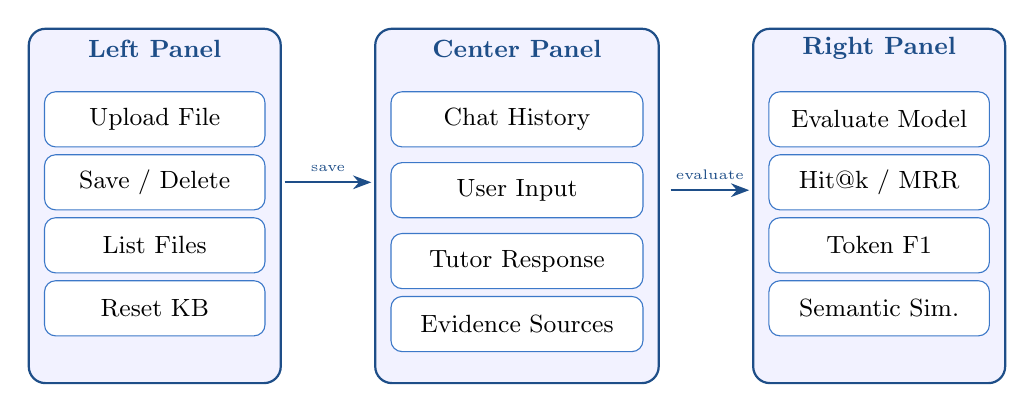
\begin{tikzpicture}[
  panel/.style={draw=primary, fill=blue!5, rounded corners=6pt,
                minimum width=3.2cm, minimum height=4.5cm, thick},
  module/.style={draw=secondary, fill=white, rounded corners=4pt,
                 minimum width=2.8cm, minimum height=0.7cm,
                 font=\small, align=center},
  arrow/.style={-{Stealth}, thick, color=primary},
  label/.style={font=\bfseries\small\color{primary}}
]

% Left panel
\node[panel] (left) at (0,0) {};
\node[label] at (0, 2.0) {Left Panel};
\node[module] at (0,  1.1) {Upload File};
\node[module] at (0,  0.3) {Save / Delete};
\node[module] at (0, -0.5) {List Files};
\node[module] at (0, -1.3) {Reset KB};

% Center panel
\node[panel, minimum width=3.6cm] (center) at (4.6,0) {};
\node[label] at (4.6, 2.0) {Center Panel};
\node[module, minimum width=3.2cm] at (4.6,  1.1) {Chat History};
\node[module, minimum width=3.2cm] at (4.6,  0.2) {User Input};
\node[module, minimum width=3.2cm] at (4.6, -0.7) {Tutor Response};
\node[module, minimum width=3.2cm] at (4.6, -1.5) {Evidence Sources};

% Right panel
\node[panel] (right) at (9.2,0) {};
\node[label] at (9.2, 2.0) {Right Panel};
\node[module] at (9.2,  1.1) {Evaluate Model};
\node[module] at (9.2,  0.3) {Hit@k / MRR};
\node[module] at (9.2, -0.5) {Token F1};
\node[module] at (9.2, -1.3) {Semantic Sim.};

% Arrows between panels
\draw[arrow] (1.65, 0.3) -- (2.75, 0.3) node[midway, above, font=\tiny] {save};
\draw[arrow] (6.55, 0.2) -- (7.55, 0.2) node[midway, above, font=\tiny] {evaluate};

\end{tikzpicture}
\caption{Three-panel Streamlit UI architecture.}
\label{fig:ui}
\end{figure}

\begin{longtable}{|p{0.28\linewidth}|p{0.65\linewidth}|}
\hline
\textbf{File} & \textbf{Responsibility} \\
\hline
\texttt{app.py} & Streamlit UI, session state, panel layout, button logic. \\
\hline
\texttt{database.py} & File parsing, chunking, embedding ingestion, hybrid retrieval, delete/reset. \\
\hline
\texttt{tutor\_engine.py} & OpenAI calls, chitchat detection, grounding checks, fallback behavior. \\
\hline
\texttt{evaluation.py} & Golden dataset loading, Hit@k, MRR, Token F1, Semantic Similarity. \\
\hline
\texttt{config.py} & Runtime constants and environment variable mapping. \\
\hline
\texttt{docker-compose.yml} / \texttt{Dockerfile} & Containerized deployment with named volumes. \\
\hline
\end{longtable}

\subsection{Ingestion Pipeline}

\begin{enumerate}[leftmargin=*]
  \item User uploads a file (\texttt{.txt}, \texttt{.md}, \texttt{.pdf}, \texttt{.csv}, \texttt{.json}).
  \item The file is parsed into clean plain text using format-specific readers.
  \item Text is split into overlapping chunks using a recursive character splitter
        (chunk size: 450, overlap: 80).
  \item Chunks are embedded with \texttt{sentence-transformers/all-MiniLM-L6-v2} and
        stored in ChromaDB with stable IDs to prevent duplicate insertion.
\end{enumerate}

\begin{figure}[h!]
\centering
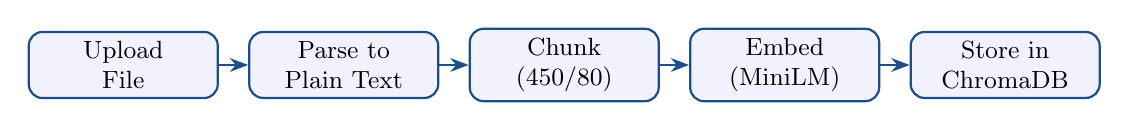
\begin{tikzpicture}[
  box/.style={draw=primary, fill=blue!5, rounded corners=5pt,
              minimum width=2.4cm, minimum height=0.8cm,
              font=\small, align=center, thick},
  arrow/.style={-{Stealth}, thick, color=primary}
]
\node[box] (upload)  at (0,0)    {Upload\\File};
\node[box] (parse)   at (2.8,0)  {Parse to\\Plain Text};
\node[box] (chunk)   at (5.6,0)  {Chunk\\(450/80)};
\node[box] (embed)   at (8.4,0)  {Embed\\(MiniLM)};
\node[box] (store)   at (11.2,0) {Store in\\ChromaDB};

\draw[arrow] (upload) -- (parse);
\draw[arrow] (parse)  -- (chunk);
\draw[arrow] (chunk)  -- (embed);
\draw[arrow] (embed)  -- (store);
\end{tikzpicture}
\caption{Document ingestion pipeline.}
\label{fig:ingestion}
\end{figure}

\subsection{Retrieval and Answer Pipeline}

\begin{enumerate}[leftmargin=*]
  \item User sends a message.
  \item If the message is chitchat (greeting, thanks, goodbye), it is answered directly
        without retrieval.
  \item Otherwise, top-k chunks are retrieved using MMR (Maximal Marginal Relevance)
        and reranked with a hybrid score:
        $0.7 \times \text{semantic rank} + 0.3 \times \text{lexical overlap}$.
  \item A grounding strength score is computed. If below 0.18, the system declines
        to answer rather than risk hallucination.
  \item An extractive answer is attempted first. If successful, it is returned directly.
        Otherwise, the full context and chat history are sent to the OpenAI API.
  \item The answer and retrieved evidence metadata (source, page, chunk) are returned.
\end{enumerate}

\begin{figure}[h!]
\centering
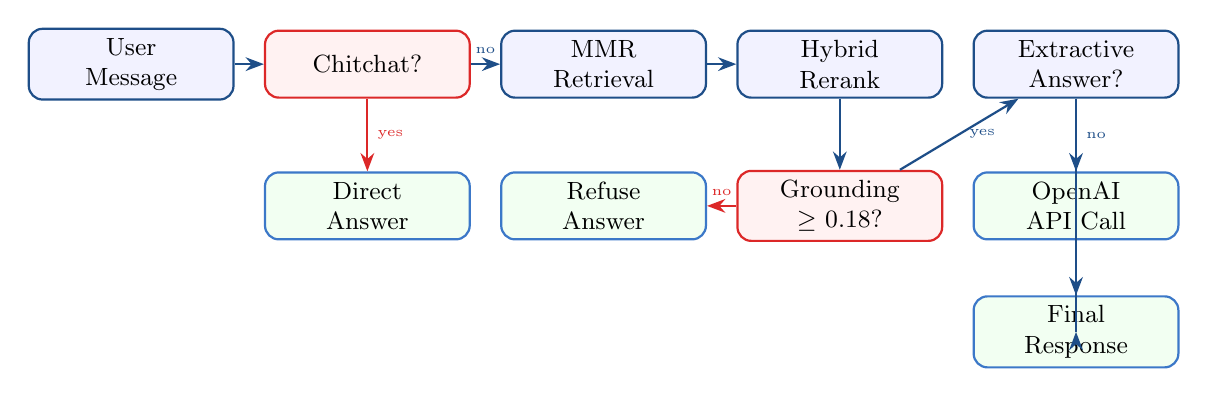
\begin{tikzpicture}[
  box/.style={draw=primary, fill=blue!5, rounded corners=5pt,
              minimum width=2.6cm, minimum height=0.85cm,
              font=\small, align=center, thick},
  decision/.style={draw=accent, fill=red!5, rounded corners=5pt,
                   minimum width=2.6cm, minimum height=0.85cm,
                   font=\small, align=center, thick},
  answer/.style={draw=secondary, fill=green!5, rounded corners=5pt,
                 minimum width=2.6cm, minimum height=0.85cm,
                 font=\small, align=center, thick},
  arrow/.style={-{Stealth}, thick, color=primary},
  redarrow/.style={-{Stealth}, thick, color=accent},
  note/.style={font=\tiny\color{gray}}
]

\node[box]      (input)     at (0, 0)     {User\\Message};
\node[decision] (chitchat)  at (3, 0)     {Chitchat?};
\node[answer]   (direct)    at (3, -1.8)  {Direct\\Answer};
\node[box]      (mmr)       at (6, 0)     {MMR\\Retrieval};
\node[box]      (rerank)    at (9, 0)     {Hybrid\\Rerank};
\node[decision] (grounding) at (9, -1.8)  {Grounding\\$\geq$ 0.18?};
\node[answer]   (refuse)    at (6, -1.8)  {Refuse\\Answer};
\node[box]      (extract)   at (12, 0)    {Extractive\\Answer?};
\node[answer]   (llm)       at (12, -1.8) {OpenAI\\API Call};
\node[answer]   (response)  at (12, -3.4) {Final\\Response};

\draw[arrow]    (input)     -- (chitchat);
\draw[redarrow] (chitchat)  -- node[right, note]{yes} (direct);
\draw[arrow]    (chitchat)  -- node[above, note]{no}  (mmr);
\draw[arrow]    (mmr)       -- (rerank);
\draw[arrow]    (rerank)    -- (grounding);
\draw[redarrow] (grounding) -- node[above, note]{no}  (refuse);
\draw[arrow]    (grounding) -- node[right, note]{yes} (extract);
\draw[arrow]    (extract)   -- node[right, note]{no}  (llm);
\draw[arrow]    (llm)       -- (response);
\draw[arrow]    (extract)   -- ++(0, -3.4) -- (response);

\end{tikzpicture}
\caption{Retrieval and answer generation pipeline.}
\label{fig:retrieval}
\end{figure}

\subsection{Persistence}

Named Docker volumes (\texttt{aitutor\_chroma\_data}, \texttt{aitutor\_uploads}) store
the ChromaDB database and uploaded files independently of the source code. This ensures
knowledge persists across container restarts and avoids accidental preloading from
the local project folder.

% ════════════════════════════════════════════════════════════════════
\section{Implementation}

\subsection{Hybrid Reranker}

The reranker in \texttt{database.py} combines two signals: the inverse rank from MMR
retrieval (semantic) and the token overlap ratio between the query and the chunk
(lexical). After scoring, duplicate chunks sharing the same \texttt{(source, chunk\_id)}
pair are removed before returning the top-k results. This improves precision for
keyword-heavy study material where pure semantic similarity may miss exact terms.

\begin{lstlisting}[caption={Hybrid reranking score in database.py}]
def _hybrid_rerank(self, query, docs, top_k):
    q_tokens = self._tokenize(query)
    scored = []
    for rank, doc in enumerate(docs, start=1):
        d_tokens = self._tokenize(doc.page_content)
        lexical = len(q_tokens.intersection(d_tokens)) / max(1, len(q_tokens))
        semantic = 1.0 / rank
        score = 0.7 * semantic + 0.3 * lexical
        scored.append((score, doc))
    scored.sort(key=lambda x: x[0], reverse=True)
    # Deduplicate by (source, chunk_id)
    unique, seen = [], set()
    for _, doc in scored:
        key = (doc.metadata.get("source"), doc.metadata.get("chunk_id"))
        if key not in seen:
            seen.add(key)
            unique.append(doc)
        if len(unique) >= top_k:
            break
    return unique
\end{lstlisting}

\subsection{Grounding Check}

Before calling the LLM, \texttt{tutor\_engine.py} first strips source-header lines
from the context via \texttt{\_extract\_clean\_context()}, then computes term overlap
between the query and the cleaned context. If the score falls below 0.18, the system
returns a refusal message. Note that an extractive answer is always attempted first;
the grounding check only runs if the extractive step returns nothing.

\begin{lstlisting}[caption={Grounding strength check in tutor\_engine.py}]
def _grounding_strength(self, question, context):
    clean_context = self._extract_clean_context(context)
    if not clean_context:
        return 0.0
    q_terms = {t for t in re.findall(r"\w+", question.lower()) if len(t) > 2}
    c_terms = {t for t in re.findall(r"\w+", clean_context.lower()) if len(t) > 2}
    if not q_terms or not c_terms:
        return 0.0
    return len(q_terms.intersection(c_terms)) / max(1, len(q_terms))
\end{lstlisting}

\subsection{Supported File Formats}

\begin{itemize}[leftmargin=*]
  \item \texttt{.txt}, \texttt{.md}: direct UTF-8 text read.
  \item \texttt{.pdf}: page text extraction via PyPDF2.
  \item \texttt{.csv}: rows flattened to pipe-separated text lines.
  \item \texttt{.json}: nested objects recursively flattened to \texttt{key: value} lines.
\end{itemize}

% ════════════════════════════════════════════════════════════════════
\section{Evaluation Framework}

\subsection{Golden Dataset}

A JSONL file (\texttt{golden\_dataset.jsonl}) contains evaluation samples, each with
a \texttt{question}, a reference \texttt{answer}, and the expected \texttt{source}
filename.

\subsection{Metrics}

\begin{longtable}{|p{0.25\linewidth}|p{0.68\linewidth}|}
\hline
\textbf{Metric} & \textbf{Description} \\
\hline
Hit@k & Whether the expected source file appears in the top-k retrieved chunks. \\
\hline
MRR & Mean Reciprocal Rank: measures how highly the expected source is ranked. \\
\hline
Token F1 & Lexical overlap (precision/recall) between generated and reference answers. \\
\hline
Semantic Similarity & Cosine similarity between embeddings of generated and reference answers. \\
\hline
\end{longtable}

These metrics together assess both \textit{retrieval quality} (Hit@k, MRR) and
\textit{generation quality} (Token F1, Semantic Similarity), providing a complete
picture of system performance.

\begin{infobox}{Sample Evaluation Output}
\begin{verbatim}
Samples: 10   Hit@1: 0.80   Hit@3: 0.90   MRR: 0.843
Answer F1 (avg): 0.61       Semantic Similarity (avg): 0.74
\end{verbatim}
\end{infobox}

% ════════════════════════════════════════════════════════════════════
\section{Discussion: Mimicking vs.\ Understanding}
\label{sec:discussion}

A key question raised in the course is how far chatbot techniques can go, and what
distinguishes mimicking from actual understanding.

This system retrieves relevant text chunks and selects sentences with high keyword
overlap. It does not parse meaning, draw inferences, or build a conceptual model of
the material. In that sense it is firmly on the \textit{mimicking} side: it
pattern-matches queries to stored text.

However, the grounding mechanism adds a layer of epistemic caution: the system
refuses to answer when evidence is weak, which is closer to how a careful human
would behave under uncertainty. The LLM component adds fluency and some degree of
paraphrase, but the underlying knowledge still comes entirely from retrieved text.

This illustrates a practical boundary: RAG systems can produce useful, grounded
responses without understanding, but they cannot reason beyond what is explicitly
present in the retrieved context.

% ════════════════════════════════════════════════════════════════════
\section{Known Limitations}

\begin{itemize}[leftmargin=*]
  \item Scanned PDFs without a text layer return empty content; OCR is not supported.
  \item Semantic evaluation is embedding-based only; an LLM-judge could provide
        deeper quality assessment.
  \item Several LangChain APIs used are deprecated and should be upgraded.
  \item DOCX and other formats are not yet supported.
  \item The \texttt{generate\_quiz()} function has no \texttt{max\_tokens} limit,
        risking unbounded API cost.
  \item Uploaded filenames are not sanitized before use in file paths, creating a
        potential path traversal vulnerability.
\end{itemize}

% ════════════════════════════════════════════════════════════════════
\section{Conclusion}

This project successfully implements a RAG-based educational assistant that extends
the course concept of conversational AI by adding hybrid retrieval reranking, grounding
checks, persistent memory, and a quantitative evaluation framework. All main objectives
were met: the system provides grounded answers, persists knowledge across restarts,
allows file-level memory management, and measures its own performance.

The discussion of mimicking vs.\ understanding reveals that the system is effective
precisely because it avoids hallucination through grounding, not because it understands
the material. This is both its strength and its fundamental limitation.

Future work includes OCR support for scanned PDFs, DOCX ingestion, LLM-judge
evaluation, and upgrading vulnerable dependencies.

% ════════════════════════════════════════════════════════════════════
\newpage
\section*{Appendix: Key Implementation Components}
\addcontentsline{toc}{section}{Appendix: Key Implementation Components}

\subsection*{Document Ingestion}
\begin{lstlisting}[caption={Chunking and storing documents in database.py}]
def process_and_store_file(self, file_path):
    filename = os.path.basename(file_path)
    raw_text = self._load_file_text(file_path)
    if not raw_text:
        return 0
    base_doc = Document(page_content=raw_text,
                        metadata={"source": filename, "page": 1})
    chunks = self.text_splitter.split_documents([base_doc])
    ids = []
    for idx, chunk in enumerate(chunks):
        chunk.metadata["chunk_id"] = idx
        stable = re.sub(r"[^a-zA-Z0-9_.-]", "_", filename.lower())
        ids.append(f"{stable}::chunk::{idx}")
    self.vector_store.add_documents(chunks, ids=ids)
    return len(chunks)
\end{lstlisting}

\subsection*{Evaluation Pipeline}
\begin{lstlisting}[caption={Token F1 and semantic similarity in evaluation.py}]
def _token_f1(prediction, reference):
    pred_tokens = _normalize(prediction)
    ref_tokens  = _normalize(reference)
    common = sum(min(pred_tokens.count(t), ref_tokens.count(t))
                 for t in set(pred_tokens))
    if common == 0:
        return 0.0
    precision = common / len(pred_tokens)
    recall    = common / len(ref_tokens)
    return 2 * precision * recall / (precision + recall)

def _semantic_similarity(prediction, reference):
    embedder = _get_semantic_embedder()
    vectors  = embedder.embed_documents([prediction, reference])
    return _cosine_similarity(vectors[0], vectors[1])
\end{lstlisting}

\subsection*{Response Generation}
\begin{lstlisting}[caption={Grounded response logic in tutor\_engine.py}]
def get_response(self, user_input, record_memory=True):
    if self._is_chitchat(user_input):
        return self._chitchat_answer(user_input)

    context   = self._retrieve_context(user_input)
    grounding = self._grounding_strength(user_input, context)

    # Extractive answer is attempted first
    if context.strip():
        extractive = self._extractive_answer(user_input, context)
        if extractive:
            return extractive

    # Grounding check before calling the LLM
    if context.strip() and grounding < 0.18:
        return ("I don't have enough evidence in the retrieved context "
                "to answer confidently.")

    response = self.client.chat.completions.create(
        model=config.OPENAI_MODEL,
        temperature=config.OPENAI_TEMPERATURE,
        max_tokens=config.OPENAI_MAX_OUTPUT_TOKENS,
        messages=[
            {"role": "system", "content": "You are a precise educational tutor."},
            {"role": "user",   "content": self._build_prompt(user_input, context)},
        ],
    )
    return self._trim_to_two_sentences(
        response.choices[0].message.content.strip())
\end{lstlisting}



\newpage
\section*{Appendix: Full Implementation Components}
\addcontentsline{toc}{section}{Appendix: Full Implementation Components}

\subsection*{Document Ingestion}
\begin{lstlisting}[caption={app.py}]
import os
import streamlit as st

import config
from audio_processor import AudioProcessor
from database import DocumentProcessor
from evaluation import evaluate_dataset, load_golden_dataset
from tutor_engine import TutorEngine
\end{lstlisting}

\subsection*{Configuration}
\begin{lstlisting}[caption={config.py}]
import os
from dotenv import load_dotenv

load_dotenv()

BASE_DIR = os.path.dirname(os.path.abspath(__file__))

TEMP_UPLOAD_DIR = os.path.join(BASE_DIR, "temp_uploads")
CHROMA_DB_DIR = os.path.join(BASE_DIR, "chroma_db")
DB_DIR = CHROMA_DB_DIR

COLLECTION_NAME = "course_documents"
EMBEDDING_MODEL_NAME = "sentence-transformers/all-MiniLM-L6-v2"

CHUNK_SIZE = 450
CHUNK_OVERLAP = 80
DEFAULT_RETRIEVAL_K = 4
RETRIEVAL_FETCH_K_FACTOR = 4

OPENAI_MODEL = os.getenv("OPENAI_MODEL", "gpt-4o-mini")
OPENAI_API_KEY = os.getenv("OPENAI_API_KEY")
OPENAI_TEMPERATURE = float(os.getenv("OPENAI_TEMPERATURE", "0.1"))
OPENAI_MAX_OUTPUT_TOKENS = int(os.getenv("OPENAI_MAX_OUTPUT_TOKENS", "220"))
\end{lstlisting}

\subsection*{Database Module}
\begin{lstlisting}[caption={database.py}]
import os
import re
import csv
import json
from typing import Dict, List
from PyPDF2 import PdfReader
from langchain_text_splitters import RecursiveCharacterTextSplitter
from langchain_community.embeddings import HuggingFaceEmbeddings
from langchain_community.vectorstores import Chroma
from langchain_core.documents import Document

import config

class DocumentProcessor:
    def __init__(self):
        # Setup Embeddings
        self.embeddings = HuggingFaceEmbeddings(
             model_name=config.EMBEDDING_MODEL_NAME,
             model_kwargs={"device": "cpu"}
        )
        
        # Setup Persistent Vector Database (Chroma)
        self.vector_store = Chroma(
            collection_name="ai_tutor_knowledge_base",
            embedding_function=self.embeddings,
            persist_directory=config.DB_DIR
        )

        # Setup Text Splitter
        self.text_splitter = RecursiveCharacterTextSplitter(
            chunk_size=config.CHUNK_SIZE,
            chunk_overlap=config.CHUNK_OVERLAP,
            length_function=len,
        )

    def _read_txt_like(self, file_path: str) -> str:
        with open(file_path, "r", encoding="utf-8", errors="ignore") as f:
            return f.read().strip()

    def _read_pdf(self, file_path: str) -> str:
        text_parts: List[str] = []
        try:
            reader = PdfReader(file_path)
            for page in reader.pages:
                page_text = (page.extract_text() or "").strip()
                if page_text:
                    text_parts.append(page_text)
        except Exception:
            return ""
        return "\n\n".join(text_parts).strip()

    def _read_csv(self, file_path: str) -> str:
        lines: List[str] = []
        try:
            with open(file_path, "r", encoding="utf-8", errors="ignore", newline="") as f:
                reader = csv.reader(f)
                for row in reader:
                    clean_row = [c.strip() for c in row if c and c.strip()]
                    if clean_row:
                        lines.append(" | ".join(clean_row))
        except Exception:
            return ""
        return "\n".join(lines).strip()

    def _flatten_json(self, obj, prefix: str = "") -> List[str]:
        lines: List[str] = []
        if isinstance(obj, dict):
            for k, v in obj.items():
                key = f"{prefix}.{k}" if prefix else str(k)
                lines.extend(self._flatten_json(v, key))
        elif isinstance(obj, list):
            for i, item in enumerate(obj):
                key = f"{prefix}[{i}]"
                lines.extend(self._flatten_json(item, key))
        else:
            value = str(obj).strip()
            if value:
                lines.append(f"{prefix}: {value}" if prefix else value)
        return lines

    def _read_json(self, file_path: str) -> str:
        try:
            with open(file_path, "r", encoding="utf-8", errors="ignore") as f:
                data = json.load(f)
        except Exception:
            return ""
        return "\n".join(self._flatten_json(data)).strip()

    def _load_file_text(self, file_path: str) -> str:
        ext = os.path.splitext(file_path)[1].lower()
        if ext in {".txt", ".md"}:
            return self._read_txt_like(file_path)
        if ext == ".pdf":
            return self._read_pdf(file_path)
        if ext == ".csv":
            return self._read_csv(file_path)
        if ext == ".json":
            return self._read_json(file_path)
        return ""

    def process_and_store_file(self, file_path: str) -> int:
        filename = os.path.basename(file_path)
        raw_text = self._load_file_text(file_path)

        if not raw_text:
            return 0

        base_doc = Document(
            page_content=raw_text,
            metadata={"source": filename, "page": 1}
        )

        chunks: List[Document] = self.text_splitter.split_documents([base_doc])
        ids: List[str] = []
        for idx, chunk in enumerate(chunks):
            chunk.metadata["chunk_id"] = idx
            stable_source = re.sub(r"[^a-zA-Z0-9_.-]", "_", filename.lower())
            ids.append(f"{stable_source}::chunk::{idx}")

        self.vector_store.add_documents(chunks, ids=ids)
        return len(chunks)

    def _tokenize(self, text: str) -> set:
        return {t for t in re.findall(r"\w+", text.lower()) if len(t) > 2}

    def _hybrid_rerank(self, query: str, docs: List[Document], top_k: int) -> List[Document]:
        if not docs:
            return []

        q_tokens = self._tokenize(query)
        scored = []
        for rank, doc in enumerate(docs, start=1):
            d_tokens = self._tokenize(doc.page_content)
            lexical = 0.0
            if q_tokens and d_tokens:
                lexical = len(q_tokens.intersection(d_tokens)) / max(1, len(q_tokens))

            semantic = 1.0 / rank
            score = 0.7 * semantic + 0.3 * lexical
            scored.append((score, doc))

        scored.sort(key=lambda x: x[0], reverse=True)

        unique_docs: List[Document] = []
        seen = set()
        for _, doc in scored:
            source = doc.metadata.get("source", "")
            chunk_id = doc.metadata.get("chunk_id", "")
            key = (source, chunk_id)
            if key in seen:
                continue
            seen.add(key)
            unique_docs.append(doc)
            if len(unique_docs) >= top_k:
                break
        return unique_docs

    def get_retriever(self, search_k: int = None):
        if search_k is None:
            search_k = config.DEFAULT_RETRIEVAL_K
        fetch_k = max(8, search_k * config.RETRIEVAL_FETCH_K_FACTOR)
        return self.vector_store.as_retriever(
            search_type="mmr",
            search_kwargs={"k": search_k, "fetch_k": fetch_k}
        )

    def retrieve_docs(self, query: str, k: int = None) -> List[Document]:
        if k is None:
            k = config.DEFAULT_RETRIEVAL_K
        fetch_k = max(8, k * config.RETRIEVAL_FETCH_K_FACTOR)
        retriever = self.vector_store.as_retriever(
            search_type="mmr",
            search_kwargs={"k": fetch_k, "fetch_k": fetch_k}
        )
        try:
            docs = retriever.get_relevant_documents(query)
            return self._hybrid_rerank(query, docs, top_k=k)
        except Exception:
            return []

    def list_saved_files(self) -> List[Dict[str, int]]:
        try:
            payload = self.vector_store.get(include=["metadatas"])
        except Exception:
            return []

        metadatas = payload.get("metadatas", []) if isinstance(payload, dict) else []
        counts: Dict[str, int] = {}
        for md in metadatas:
            if not isinstance(md, dict):
                continue
            source = str(md.get("source", "")).strip()
            if not source:
                continue
            counts[source] = counts.get(source, 0) + 1

        rows = [{"source": k, "chunk_count": v} for k, v in counts.items()]
        rows.sort(key=lambda x: x["source"].lower())
        return rows

    def delete_source(self, source: str) -> int:
        ids = self._ids_for_source(source)
        if not ids:
            return 0
        try:
            self.vector_store.delete(ids=ids)
            return len(ids)
        except Exception:
            return 0

    def clear_all_documents(self) -> int:
        try:
            payload = self.vector_store.get(include=[])
        except Exception:
            return 0

        if not isinstance(payload, dict):
            return 0
        ids = payload.get("ids", []) or []
        if not ids:
            return 0
        try:
            self.vector_store.delete(ids=ids)
            return len(ids)
        except Exception:
            return 0
\end{lstlisting}

\subsection*{Evaluation Module}
\begin{lstlisting}[caption={evaluation.py}]
import json
import os
import re
from typing import Dict, List, Tuple
from math import sqrt

from langchain_community.embeddings import HuggingFaceEmbeddings

import config

_SEMANTIC_EMBEDDER = None

def load_golden_dataset(path: str) -> List[Dict[str, str]]:
    if not os.path.exists(path):
        return []

    rows: List[Dict[str, str]] = []
    with open(path, "r", encoding="utf-8") as f:
        for line in f:
            line = line.strip()
            if not line:
                continue
            try:
                item = json.loads(line)
            except json.JSONDecodeError:
                continue

            question = str(item.get("question", "")).strip()
            answer = str(item.get("answer", "")).strip()
            source = str(item.get("source", "")).strip()
            if question and answer:
                rows.append({
                    "question": question,
                    "answer": answer,
                    "source": source,
                })
    return rows

def _normalize(text: str) -> List[str]:
    text = text.lower()
    text = re.sub(r"[^\w\s]", " ", text)
    return [t for t in text.split() if t]

def _token_f1(prediction: str, reference: str) -> float:
    pred_tokens = _normalize(prediction)
    ref_tokens = _normalize(reference)
    if not pred_tokens or not ref_tokens:
        return 0.0

    pred_counts: Dict[str, int] = {}
    ref_counts: Dict[str, int] = {}
    for t in pred_tokens:
        pred_counts[t] = pred_counts.get(t, 0) + 1
    for t in ref_tokens:
        ref_counts[t] = ref_counts.get(t, 0) + 1

    common = 0
    for token, p_count in pred_counts.items():
        if token in ref_counts:
            common += min(p_count, ref_counts[token])

    if common == 0:
        return 0.0

    precision = common / len(pred_tokens)
    recall = common / len(ref_tokens)
    return 2 * precision * recall / (precision + recall)

def _get_semantic_embedder():
    global _SEMANTIC_EMBEDDER
    if _SEMANTIC_EMBEDDER is None:
        _SEMANTIC_EMBEDDER = HuggingFaceEmbeddings(
            model_name=config.EMBEDDING_MODEL_NAME,
            model_kwargs={"device": "cpu"},
        )
    return _SEMANTIC_EMBEDDER

def _cosine_similarity(a: List[float], b: List[float]) -> float:
    if not a or not b or len(a) != len(b):
        return 0.0
    dot = sum(x * y for x, y in zip(a, b))
    na = sqrt(sum(x * x for x in a))
    nb = sqrt(sum(y * y for y in b))
    if na == 0.0 or nb == 0.0:
        return 0.0
    return dot / (na * nb)

def _semantic_similarity(prediction: str, reference: str) -> float:
    if not prediction.strip() or not reference.strip():
        return 0.0
    try:
        embedder = _get_semantic_embedder()
        vectors = embedder.embed_documents([prediction, reference])
        return _cosine_similarity(vectors[0], vectors[1])
    except Exception:
        return 0.0

def evaluate_dataset(doc_processor, tutor_engine, dataset: List[Dict[str, str]], k_values: Tuple[int, ...] = (1, 3, 5)) -> Dict:
    if not dataset:
        return {
            "num_samples": 0,
            "hit_rates": {f"Hit@{k}": 0.0 for k in k_values},
            "mrr": 0.0,
            "avg_f1": 0.0,
            "avg_semantic_similarity": 0.0,
            "rows": [],
        }

    hit_counts = {k: 0 for k in k_values}
    mrr_total = 0.0
    f1_total = 0.0
    semantic_total = 0.0
    rows = []

    max_k = max(k_values)

    for sample in dataset:
        question = sample["question"]
        expected_answer = sample["answer"]
        expected_source = sample.get("source", "")

        docs = doc_processor.retrieve_docs(question, k=max_k)
        retrieved_sources = [str(d.metadata.get("source", "")) for d in docs]

        rank = None
        if expected_source:
            for idx, src in enumerate(retrieved_sources, start=1):
                if src == expected_source:
                    rank = idx
                    break

            for k in k_values:
                if rank is not None and rank <= k:
                    hit_counts[k] += 1
            if rank is not None:
                mrr_total += 1.0 / rank

        predicted_answer = tutor_engine.get_response(question, record_memory=False)
        f1_score = _token_f1(predicted_answer, expected_answer)
        semantic_sim = _semantic_similarity(predicted_answer, expected_answer)
        f1_total += f1_score
        semantic_total += semantic_sim

        rows.append({
            "question": question,
            "expected_source": expected_source,
            "retrieved_top1": retrieved_sources[0] if retrieved_sources else "",
            "rank_of_expected_source": rank if rank is not None else "not_found",
            "answer_f1": round(f1_score, 3),
            "semantic_similarity": round(semantic_sim, 3),
        })

    n = len(dataset)
    hit_rates = {f"Hit@{k}": round(hit_counts[k] / n, 3) for k in k_values}
    mrr = round(mrr_total / n, 3)
    avg_f1 = round(f1_total / n, 3)
    avg_semantic_similarity = round(semantic_total / n, 3)

    return {
        "num_samples": n,
        "hit_rates": hit_rates,
        "mrr": mrr,
        "avg_f1": avg_f1,
        "avg_semantic_similarity": avg_semantic_similarity,
        "rows": rows,
    }

\subsection*{Main Application}
\begin{lstlisting}[caption={app.py (continued)}]


if "doc_processor" not in st.session_state:
    st.session_state.doc_processor = DocumentProcessor()
if "tutor_engine" not in st.session_state:
    st.session_state.tutor_engine = TutorEngine(
        retriever=st.session_state.doc_processor.get_retriever(
            search_k=config.DEFAULT_RETRIEVAL_K
        )
    )
if "audio_processor" not in st.session_state:
    st.session_state.audio_processor = AudioProcessor()
if "messages" not in st.session_state:
    st.session_state.messages = [
        {
            "role": "assistant",
            "content": "Hello! I am your Socratic AI Tutor. Ask me any question about your uploaded study files.",
        }
    ]
if "retrieval_k" not in st.session_state:
    st.session_state.retrieval_k = config.DEFAULT_RETRIEVAL_K

st.set_page_config(page_title="Socratic AI Tutor", page_icon="graduation", layout="wide")
st.title("Socratic AI Tutor with Persistent Memory")

def render_evaluation_results():
    eval_result = st.session_state.get("eval_result")
    if not eval_result:
        st.info("No evaluation result yet. Click 'Evaluate Model' first.")
        return

    if eval_result["num_samples"] == 0:
        st.info(
            "No golden dataset found. Create 'golden_dataset.jsonl' in the project root to run evaluation."
        )
    else:
        c1, c2, c3, c4 = st.columns(4)
        c1.metric("Samples", eval_result["num_samples"])
        c2.metric("Hit@1", eval_result["hit_rates"]["Hit@1"])
        c3.metric("Hit@3", eval_result["hit_rates"]["Hit@3"])
        c4.metric("MRR", eval_result["mrr"])
        st.metric("Answer F1 (avg)", eval_result["avg_f1"])
        st.metric("Semantic Similarity (avg)", eval_result.get("avg_semantic_similarity", 0.0))
        st.dataframe(eval_result["rows"], use_container_width=True, height=360)

def render_saved_files_panel():
    st.subheader("Saved Files")
    saved_files = st.session_state.doc_processor.list_saved_files()
    if not saved_files:
        st.caption("No files saved yet.")
        return
    for row in saved_files:
        c1, c2 = st.columns([0.88, 0.12], gap="small")
        c1.markdown(f"`{row['source']}`  ({row['chunk_count']} chunks)")
        if c2.button("X", key=f"delete_{row['source']}", help="Delete this file", use_container_width=True):
            deleted = st.session_state.doc_processor.delete_source(row["source"])
            st.session_state.tutor_engine.update_retriever(
                st.session_state.doc_processor.get_retriever(
                    search_k=st.session_state.retrieval_k
                )
            )
            if deleted > 0:
                st.success(f"Deleted `{row['source']}` ({deleted} chunks)")
            else:
                st.warning(f"Could not delete `{row['source']}`")
            st.rerun()

left_col, center_col, right_col = st.columns([1.0, 1.8, 1.0], gap="large")

with left_col:
    st.header("Knowledge Base")
    st.write("Upload study files, save them, and see what is currently stored.")

    retrieval_k = st.slider(
        "Retrieval Top-k",
        min_value=1,
        max_value=8,
        value=st.session_state.retrieval_k,
        help="Lower values are stricter; higher values provide broader context.",
        key="left_retrieval_k",
    )
    if retrieval_k != st.session_state.retrieval_k:
        st.session_state.retrieval_k = retrieval_k
        st.session_state.tutor_engine.update_retriever(
            st.session_state.doc_processor.get_retriever(
                search_k=st.session_state.retrieval_k
            )
        )

    uploaded_file = st.file_uploader(
        "Upload a file",
        type=["txt", "md", "pdf", "csv", "json"],
        key="left_file_uploader",
    )
    if st.button("Process & Save Document", key="left_save_btn") and uploaded_file:
        with st.spinner("Processing document..."):
            temp_path = os.path.join(config.TEMP_UPLOAD_DIR, uploaded_file.name)
            with open(temp_path, "wb") as f:
                f.write(uploaded_file.getbuffer())

            num_chunks = st.session_state.doc_processor.process_and_store_file(temp_path)
            st.session_state.tutor_engine.update_retriever(
                st.session_state.doc_processor.get_retriever(
                    search_k=st.session_state.retrieval_k
                )
            )

            if num_chunks == 0:
                st.warning("File was empty or unsupported. Nothing was added.")
            else:
                st.success(f"Saved: `{uploaded_file.name}` ({num_chunks} chunks)")
                st.rerun()

    st.divider()
    if st.button("Reset Knowledge Base (Delete All)", key="left_reset_all_btn", type="secondary"):
        deleted_total = st.session_state.doc_processor.clear_all_documents()
        st.session_state.tutor_engine.update_retriever(
            st.session_state.doc_processor.get_retriever(
                search_k=st.session_state.retrieval_k
            )
        )
        if deleted_total > 0:
            st.success(f"All saved knowledge deleted ({deleted_total} chunks).")
        else:
            st.info("Knowledge base was already empty.")
        st.rerun()

    render_saved_files_panel()

with center_col:
    st.header("Chat")
    for msg in st.session_state.messages:
        with st.chat_message(msg["role"]):
            st.write(msg["content"])
            if msg["role"] == "assistant" and msg.get("sources"):
                source_lines = []
                for s in msg["sources"]:
                    source_lines.append(
                        f"- source: `{s.get('source', 'unknown')}`, page: `{s.get('page', '?')}`, chunk: `{s.get('chunk_id', '?')}`"
                    )
                st.markdown("Retrieved evidence:\n" + "\n".join(source_lines))

    st.divider()
    with st.form("center_chat_form", clear_on_submit=True):
        input_col, send_col = st.columns([0.86, 0.14], gap="small")
        user_input = input_col.text_input(
            "Message",
            key="center_chat_input",
            placeholder="Ask a question...",
            label_visibility="collapsed",
        )
        send_clicked = send_col.form_submit_button("Send", use_container_width=True)

    if send_clicked and user_input.strip():
        with st.spinner("Thinking..."):
            st.session_state.messages.append({"role": "user", "content": user_input.strip()})
            response_text = st.session_state.tutor_engine.get_response(user_input.strip())
            st.session_state.messages.append(
                {
                    "role": "assistant",
                    "content": response_text,
                    "sources": st.session_state.tutor_engine.get_last_retrieved_sources(),
                }
            )
        st.rerun()

with right_col:
    st.header("Assessment")
    has_saved_files = len(st.session_state.doc_processor.list_saved_files()) > 0
    st.button(
        "Generate Contextual Quiz",
        disabled=True,
        help="Coming soon (outside MVP scope).",
        key="right_quiz_btn",
    )

    dataset_path = os.path.join(config.BASE_DIR, "golden_dataset.jsonl")
    if st.button(
        "Evaluate Model",
        key="right_eval_btn",
        disabled=not has_saved_files,
        help="Save at least one file first." if not has_saved_files else None,
    ):
        with st.spinner("Running retrieval/generation evaluation..."):
            dataset = load_golden_dataset(dataset_path)
            result = evaluate_dataset(
                doc_processor=st.session_state.doc_processor,
                tutor_engine=st.session_state.tutor_engine,
                dataset=dataset,
                k_values=(1, 3, 5),
            )
            st.session_state.eval_result = result
    with st.expander("View Evaluation Results", expanded=False):
        render_evaluation_results()
\end{lstlisting}

\subsection*{Additional Files}
\begin{lstlisting}[caption={requirements.txt}]
streamlit==1.36.0
langchain==0.2.6
langchain-community==0.2.6
langchain-core==0.2.11
chromadb==0.5.3
sentence-transformers==2.7.0
pypdf2==3.0.1
python-dotenv==1.0.1
gtts==2.5.1
audio-recorder-streamlit==0.0.10
openai==1.30.5
httpx==0.27.2
\end{lstlisting}

\begin{lstlisting}[caption={test\_connection.py}]
import requests
import json

urls = [
    "http://localhost:11434/api/tags",
    "https://mitsubishi-refers-raid-rail.trycloudflare.com/api/tags"
]

for url in urls:
    print(f"Checking {url}...")
    try:
        response = requests.get(url, timeout=5)
        print(f"Status Code: {response.status_code}")
        if response.status_code == 200:
            print(f"Ollama is reachable! {response.json()}")
        else:
            print(f"Not reachable. Response: {response.text[:100]}")
    except Exception as e:
        print(f"Error: {e}")
\end{lstlisting}

\begin{lstlisting}[caption={azure-deploy.json (ARM Template)}]
{
    "$schema": "https://schema.management.azure.com/schemas/2019-04-01/deploymentTemplate.json#",
    "contentVersion": "1.0.0.0",
    "parameters": {
        "vmName": {
            "type": "string",
            "defaultValue": "ai-tutor-vm"
        },
        "adminUsername": {
            "type": "string",
            "defaultValue": "azureuser"
        },
        "adminPassword": {
            "type": "secureString"
        },
        "vmSize": {
            "type": "string",
            "defaultValue": "Standard_B2ms"
        },
        "location": {
            "type": "string",
            "defaultValue": "[resourceGroup().location]"
        }
    },
    "variables": {
        "vnetName": "[concat(parameters('vmName'), '-vnet')]",
        "nsgName": "[concat(parameters('vmName'), '-nsg')]",
        "publicIpName": "[concat(parameters('vmName'), '-pip')]"
    },
    "resources": [
        {
            "type": "Microsoft.Network/networkSecurityGroups",
            "apiVersion": "2023-09-01",
            "name": "[variables('nsgName')]",
            "location": "[parameters('location')]",
            "properties": {
                "securityRules": [
                    {
                        "name": "Allow-SSH",
                        "properties": {
                            "priority": 1000,
                            "access": "Allow",
                            "direction": "Inbound",
                            "protocol": "Tcp",
                            "destinationPortRange": "22"
                        }
                    },
                    {
                        "name": "Allow-Streamlit",
                        "properties": {
                            "priority": 1010,
                            "access": "Allow",
                            "direction": "Inbound",
                            "protocol": "Tcp",
                            "destinationPortRange": "8501"
                        }
                    }
                ]
            }
        }
    ]
}
\end{lstlisting}

\begin{lstlisting}[caption={azure-deploy.parameters.json}]
{
    "$schema": "https://schema.management.azure.com/schemas/2019-04-01/deploymentParameters.json#",
    "contentVersion": "1.0.0.0",
    "parameters": {
        "vmName": {
            "value": "ai-tutor-vm"
        },
        "adminUsername": {
            "value": "azureuser"
        },
        "adminPassword": {
            "value": "YourStrongPassword_123!"
        },
        "vmSize": {
            "value": "Standard_B2ms"
        },
        "location": {
            "value": "westeurope"
        }
    }
}
\end{lstlisting}

\begin{lstlisting}[caption={golden\_dataset.jsonl (sample)}]
{"question":"What is the main topic of chapter 1?","answer":"The main topic of chapter 1 is ...","source":"your_file_name.txt"}
{"question":"Define term X based on the text.","answer":"Term X means ...","source":"your_file_name.txt"}
{"question":"What are the two key differences between A and B?","answer":"The two key differences are ...","source":"your_file_name.txt"}
\end{lstlisting}

\subsection*{Tutor Engine Module}
\begin{lstlisting}[caption={tutor\_engine.py}]
import re

from openai import OpenAI, RateLimitError, AuthenticationError, APIConnectionError, OpenAIError
from langchain.memory import ConversationBufferMemory

import config

class TutorEngine:
    def __init__(self, retriever):
        self.client = OpenAI(api_key=config.OPENAI_API_KEY)
        self.retriever = retriever
        self.last_retrieved_sources = []
        self.memory = ConversationBufferMemory(
            memory_key="chat_history",
            return_messages=True
        )

    def _retrieve_context(self, question: str) -> str:
        try:
            docs = self.retriever.get_relevant_documents(question)
        except Exception:
            docs = []
        self.last_retrieved_sources = []
        if not docs:
            return ""
        context_parts = []
        seen = set()
        for doc in docs:
            source = doc.metadata.get("source", "unknown")
            page = doc.metadata.get("page", "?")
            chunk_id = doc.metadata.get("chunk_id", "?")
            key = (source, page, chunk_id)
            if key in seen:
                continue
            seen.add(key)
            self.last_retrieved_sources.append(
                {"source": source, "page": page, "chunk_id": chunk_id}
            )
            context_parts.append(
                f"[Source: {source}, page {page}, chunk {chunk_id}]\n{doc.page_content}"
            )
        return "\n\n".join(context_parts)

    def _extractive_answer(self, question: str, context: str) -> str:
        clean_context = self._extract_clean_context(context)
        if not clean_context:
            return ""
        question_terms = {
            t for t in re.findall(r"\w+", question.lower())
            if len(t) > 2
        }
        stop_terms = {
            "what", "when", "where", "which", "does", "about", "from", "with",
            "that", "this", "have", "your", "give", "common", "used", "mean",
            "important", "why", "is", "the", "are", "for", "and"
        }
        question_terms = {t for t in question_terms if t not in stop_terms}
        if not question_terms:
            return ""
        sentences = re.split(r"(?<=[.!?])\s+", clean_context)
        scored = []
        for sent in sentences:
            sent = sent.strip()
            if not sent:
                continue
            sent_terms = {t for t in re.findall(r"\w+", sent.lower()) if len(t) > 2}
            if not sent_terms:
                continue
            overlap = len(question_terms.intersection(sent_terms))
            if overlap == 0:
                continue
            score = overlap / max(1, len(question_terms))
            scored.append((score, sent))
        if not scored:
            return ""
        scored.sort(key=lambda x: x[0], reverse=True)
        best_score, best_sentence = scored[0]
        if best_score < 0.20:
            return ""
        return self._trim_to_two_sentences(best_sentence)

    def _grounding_strength(self, question: str, context: str) -> float:
        clean_context = self._extract_clean_context(context)
        if not clean_context:
            return 0.0
        q_terms = {t for t in re.findall(r"\w+", question.lower()) if len(t) > 2}
        c_terms = {t for t in re.findall(r"\w+", clean_context.lower()) if len(t) > 2}
        if not q_terms or not c_terms:
            return 0.0
        overlap = len(q_terms.intersection(c_terms))
        return overlap / max(1, len(q_terms))

    def get_response(self, user_input: str, record_memory: bool = True) -> str:
        if self._is_chitchat(user_input):
            self.last_retrieved_sources = []
            answer = self._chitchat_answer(user_input)
            if record_memory:
                self.memory.chat_memory.add_user_message(user_input)
                self.memory.chat_memory.add_ai_message(answer)
            return answer
        context = self._retrieve_context(user_input)
        grounding = self._grounding_strength(user_input, context)
        if context.strip():
            extractive = self._extractive_answer(user_input, context)
            if extractive:
                answer = extractive
                if record_memory:
                    self.memory.chat_memory.add_user_message(user_input)
                    self.memory.chat_memory.add_ai_message(answer)
                return answer
        if context.strip():
            if grounding < 0.18:
                answer = (
                    "I don't have enough evidence in the retrieved context to answer confidently."
                )
                if record_memory:
                    self.memory.chat_memory.add_user_message(user_input)
                    self.memory.chat_memory.add_ai_message(answer)
                return answer
        try:
            response = self.client.chat.completions.create(
                model=config.OPENAI_MODEL,
                temperature=config.OPENAI_TEMPERATURE,
                max_tokens=config.OPENAI_MAX_OUTPUT_TOKENS,
                messages=[
                    {"role": "system", "content": "You are a precise educational tutor."},
                    {"role": "user", "content": self._build_prompt(user_input, context)},
                ],
            )
            answer = self._trim_to_two_sentences((response.choices[0].message.content or "").strip())
        except OpenAIError:
            answer = self._fallback_answer(user_input, context)
        if record_memory:
            self.memory.chat_memory.add_user_message(user_input)
            self.memory.chat_memory.add_ai_message(answer)
        return answer
\end{lstlisting}

\subsection*{Audio Processor Module}
\begin{lstlisting}[caption={audio\_processor.py}]
import base64
from gtts import gTTS
import os

class AudioProcessor:
    def __init__(self):
        self.temp_audio_file = "temp_response.mp3"

    def text_to_speech_html(self, text: str, lang: str = 'en') -> str:
        # Create TTS
        tts = gTTS(text=text, lang=lang, slow=False)
        tts.save(self.temp_audio_file)

        # Read the audio file
        with open(self.temp_audio_file, "rb") as f:
            data = f.read()
            b64 = base64.b64encode(data).decode()
            
        # Create an invisible HTML audio tag that plays automatically
        md = f"""
            <audio autoplay="true" style="display:none;">
            <source src="data:audio/mp3;base64,{b64}" type="audio/mp3">
            </audio>
            """
        
        # Cleanup temp file
        if os.path.exists(self.temp_audio_file):
            os.remove(self.temp_audio_file)
            
        return md
\end{lstlisting}

\subsection*{Docker Configuration}
\begin{lstlisting}[caption={docker-compose.yml}]
services:
  aitutor:
    build: .
    container_name: socratic_ai_tutor
    ports:
      - "8501:8501"
    volumes:
      - aitutor_chroma_data:/app/chroma_db
      - aitutor_uploads:/app/temp_uploads
    env_file:
      - .env
    restart: unless-stopped

volumes:
  aitutor_chroma_data:
  aitutor_uploads:
\end{lstlisting}

\begin{lstlisting}[caption={Dockerfile}]
FROM python:3.11-slim

WORKDIR /app

ENV PYTHONDONTWRITEBYTECODE=1
ENV PYTHONUNBUFFERED=1
ENV STREAMLIT_SERVER_PORT=8501
ENV STREAMLIT_SERVER_ADDRESS=0.0.0.0

RUN apt-get update && apt-get install -y \
    build-essential \
    curl \
    && rm -rf /var/lib/apt/lists/*

COPY requirements.txt .

RUN pip install --no-cache-dir --upgrade pip && \
    pip install --no-cache-dir -r requirements.txt

COPY . .

RUN mkdir -p /app/chroma_db /app/temp_uploads

EXPOSE 8501

CMD ["streamlit", "run", "app.py", "--server.port=8501", "--server.address=0.0.0.0"]
\end{lstlisting}

\end{document}
